\documentclass[a1paper,portrait,american,fontscale=.4]{baposter}

\usepackage{lipsum}
\usepackage{listings}
\usepackage{todo}
\usepackage{hyperref}
\usepackage{qrcode}
\usepackage{float}
\usepackage{algorithm}
\usepackage{algpseudocode}
\usepackage{multicol}
\usepackage{setspace}
\usepackage{tikz}
\usetikzlibrary{
    arrows,
    arrows.meta,
    backgrounds,
    calc,
    chains,
    decorations,
    decorations.pathreplacing,
    matrix,
    positioning,
    scopes,
    shadows,
    shapes,
    shapes.multipart,
}

\definecolor{MyColorOne}{HTML}{637462}
\definecolor{MyColorTwo}{HTML}{b7af8a}
\definecolor{MyColorThree}{HTML}{ccb15a}
\colorlet{MyBoxBG}{white!96!black}

\tikzstyle{rect}=[draw,rectangle,thick,on chain,font=\tiny,inner sep=.5mm,minimum height=1.2em]
\tikzstyle{ssd}=[draw,rectangle,rounded corners,very thick,minimum width=3cm,minimum height=4cm]
\tikzstyle{ssd_screw}=[circle,fill=black!50!white,inner sep=0mm,minimum width=2mm]
\tikzstyle{memory}=[draw,rectangle,very thick,minimum width=18mm,minimum height=40mm]
\tikzstyle{file}=[draw,rectangle,minimum width=15mm,text width=15mm,minimum height=20mm,align=center]

\newcommand{\SSD}[3][]{%
    \node[ssd,#1] (#2) {#3};
    \node[below=1mm] at (#2.north) {\textbf{#2}};
    \node[ssd_screw,xshift=2mm,yshift=-2mm] at (#2.north west) {};
    \node[ssd_screw,xshift=-2mm,yshift=-2mm] at (#2.north east) {};
    \node[ssd_screw,xshift=2mm,yshift=2mm] at (#2.south west) {};
    \node[ssd_screw,xshift=-2mm,yshift=2mm] at (#2.south east) {};
}

\newcommand{\Memory}[3][]{%
    \node[memory,#1] (#2) {#3};
    \node[below=1mm,text width=15mm,align=center] at (#2.north) {\textbf{#2}};
}

\newcommand{\File}[2][]{%
    \node[file,#1] (#2)
        {%
            \ttfamily\tiny
            01000001010000\\
            11010011010010\\
            00000101001101\\
            00100101000111\\
            01001101010011\\
            11010001000010\\
            00000011001000\\
            11000000110001\\
            00111001\phantom{000000}\\

        };
    \node[above] at (#2.north) {\textbf{\footnotesize #2}};
}

\newcommand{\CPU}[3][]{%
    \node[draw,rectangle,very thick,minimum width=22mm,minimum height=22mm,#1] (#2) {};
    \node[draw,rectangle,very thick,rounded corners, minimum width=19mm,minimum height=19mm] at (#2) {#3};
    \node[below=3mm] at (#2.north) {\textbf{#2}};
}

\begin{document}
\begin{poster}{
        %----- Poster Settings -----------------------------------------------------------------------------------------
        background=none,
        columns=6,
        %----- Box Settings --------------------------------------------------------------------------------------------
        boxColorOne=MyBoxBG,
        boxshade=plain,
        headershade=shadeLR,
        headerColorOne=MyColorOne,
        headerColorTwo=MyColorTwo,
        textborder=roundedleft,
        borderColor=black,
        headerborder=open,
        headershape=roundedright,
        headerfont=\large\bfseries,
        headerFontColor=white!90!MyColorTwo,
        linewidth=0pt,
    }
    {}
    {
        \LARGE ACM~SIGMOD'19~Programming~Contest
    }
    {
        \vspace*{.5em}
        \emph{teamsic:}~Immanuel~L.~Haffner
        \qquad
        Advisor:~Jens~Dittrich
        \\[.5em]
        \small
        Big~Data~Analytics~Group, Saarland~Informatics~Campus
        \\[.5em]
        \url{bigdata.uni-saarland.de}
    }
    {
    }

    \headerbox{Task Description}{name=task,column=0,span=3}{
        \begin{center}
            \scalebox{.8}{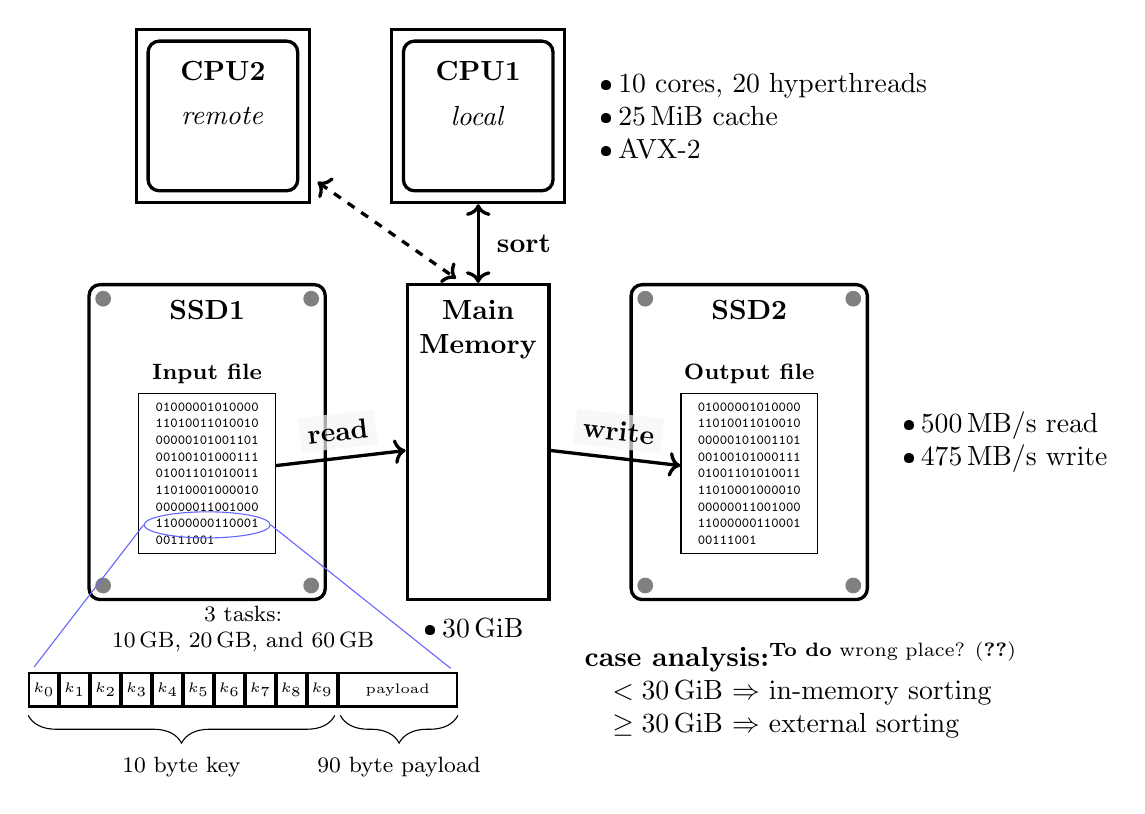
\begin{tikzpicture}
    % Hardware
    \SSD{SSD1}{};
    \Memory[right=10mm of SSD1]{Main Memory}{};
    \SSD[right=10mm of Main Memory]{SSD2}{};
    \File[anchor=south,above=6mm of SSD1.south]{Input file};
    \File[anchor=south,above=6mm of SSD2.south]{Output file};
    \draw[->,very thick] (Input file) to node[above=1mm,sloped,fill=MyBoxBG,inner sep=1mm,opacity=.7,text opacity=1] {\textbf{read}} (Main Memory);
    \draw[->,very thick] (Main Memory) to node[above=1mm,sloped,fill=MyBoxBG,inner sep=1mm,opacity=.7,text opacity=1] {\textbf{write}} (Output file);
    %\draw[->,very thick,out=255,in=285,looseness=2.5] (Main Memory) to node[below=1mm] {\textbf{sort}} (Main Memory);
    \CPU[above=of Main Memory]{CPU1}{\emph{local}};
    \draw[<->,very thick] (CPU1) -- node[right=1mm]{\textbf{sort}} (Main Memory.north);
    \CPU[left=of CPU1]{CPU2}{\emph{remote}};
    \draw[<->,very thick,dashed,shorten >=1mm,shorten <=1mm] (CPU2) -- ([xshift=-2mm]Main Memory.north);

    % Specification
    \node[right=3mm of CPU1,align=left]{%
        \textbullet\,10~cores, 20~hyperthreads
        \\
        \textbullet\,25\,MiB cache
        \\
        \textbullet\,AVX-2
    };

    \node[right=3mm of SSD2,align=left]{%
        \textbullet\,500\,MB/s read
        \\
        \textbullet\,475\,MB/s write
    };

    \node[below=1mm of Main Memory.south,align=left,anchor=north]{%
        \textbullet\,30\,GiB
    };

    \begin{scope}[start chain=going right,node distance=-.2\pgflinewidth,local bounding box=record]
        \node[rect,below left= 15mm and 10mm of Input file] (k0) {$k_0$};
        \node[rect] {$k_1$};
        \node[rect] {$k_2$};
        \node[rect] {$k_3$};
        \node[rect] {$k_4$};
        \node[rect] {$k_5$};
        \node[rect] {$k_6$};
        \node[rect] {$k_7$};
        \node[rect] {$k_8$};
        \node[rect] {$k_9$};
        \node[rect,minimum width=15mm] (payload) {payload};
    \end{scope}
    \draw[decorate,decoration={brace,mirror,amplitude=10pt,raise=1mm}]
    (k0.south west) -- node[below=5mm] {\footnotesize 10 byte key} ([xshift=-1pt]payload.south west);
    \draw[decorate,decoration={brace,mirror,amplitude=10pt,raise=1mm}]
    ([xshift=1pt]payload.south west) -- node[below=5mm] {\footnotesize 90 byte payload} (payload.south east);

    \node[ellipse,draw=blue!60,minimum height=2.6mm,minimum width=16mm] (zoom) at ([yshift=3.7mm] Input file.south) {};
    \draw[draw=blue!60,shorten >=1mm] (zoom.west) -- (record.north west);
    \draw[draw=blue!60,shorten >=1mm] (zoom.east) -- (record.north east);

    \node[above=1.5mm of record,align=center,font=\footnotesize] {3~tasks:\\10\,GB, 20\,GB, and 60\,GB};

    \node[align=left, right=15mm of record] {%
        \textbf{case analysis:}\Todo{wrong place?}
        \\
        \quad $< 30$\,GiB $\Rightarrow$ in-memory sorting
        \\
        \quad $\ge 30$\,GiB $\Rightarrow$ external sorting
    };
\end{tikzpicture}
}
        \end{center}
    }

    \headerbox{Sorting Algorithm}{name=algo,column=3,span=3}{
        \begin{itemize}
            \item in-place radix sort with \emph{American Flag Sort}
            \item parallelize on first recursion: use one thread per call (work list) or all threads per call
            \item custom concurrent American Flag Sort partitioning
            \item fall back to \texttt{std::sort()} below certain threshold (i.e.\ \emph{introsort} with fall back to
                \emph{insertion sort})
        \end{itemize}

        \begin{center}
            \includegraphics[scale=.05]{fig/parallel_AFS.jpg}
        \end{center}
    }

    \headerbox{In-Memory Sorting}{name=inmemory,column=3,span=2,below=algo}{
        \begin{itemize}
            \item \texttt{mmap()} the entire output file and read the input file into that memory region
            \item decide whether all values $[0 - 255]$ or only printable ASCII $[32-126]$ by inspection of first $10$
                records
            \item assume uniform distribution of keys
            \item already partition on first byte while reading from input file
            \item finish partitions in parallel with American Flag Sort
            \item don't write to disk; terminate the application $\rightarrow$~kernel takes care to write changed
                \texttt{mmap()}'d file back to disk
        \end{itemize}
    }

    \headerbox{External Memory Sorting}{name=external,column=0,span=3,below=task}{
        \begin{itemize}
            \item read as much data as fits into main memory
            \item sort that data with parallel American Flag Sort on NUMA region~0
            \item in parallel, partition remaining data into 256 buckets on SSD1 on NUMA region~1
            \item starting with the smallest bucket, load a bucket, sort it, then merge the bucket with the sorted in
                memory data and write it to the output file on disk
        \end{itemize}

        \begin{center}
            \includegraphics[scale=.2]{fig/external_sort_1.jpg}
            \includegraphics[scale=.2]{fig/external_sort_2.jpg}
        \end{center}

        \begin{minipage}[t][66mm][c]{.53\textwidth}
            \includegraphics[scale=.18]{fig/timeline.png}
        \end{minipage}%
        \begin{minipage}[t][66mm][c]{.47\textwidth}
            \begin{enumerate}
                \item Read the first $M - \epsilon$ records into main memory.
                \item Start to sort the $M - \epsilon$ records.
                \item[2'.] Concurrently read the remaining $N - (M - \epsilon)$ records and partition them into $256$ buckets
                    on SSD1.

                \item Load the next smallest partition into main memory.
                \item Sort the records in the partition.
                \item Merge the sorted partition with the sorted in-memory data and write to output file on SSD1.
            \end{enumerate}
        \end{minipage}
    }

    \headerbox{Third-Party Libraries}{name=libs,column=3,span=2,below=inmemory}{
        \begin{itemize}
            \item Agner Fog's \texttt{asmlib} {\footnotesize (for \texttt{memcmp()})}
            \item CTPL: Modern and Efficient C\texttt{++} Thread Pool Library {\footnotesize (not in final submission)}
            \item Intel Processor Counter Monitor (PCM) {\footnotesize (not in final submission)}
        \end{itemize}
    }

    \headerbox{Source Code}{name=code,column=3,span=2,below=libs}{
        \begin{minipage}[b]{.65\linewidth}
            The source code is available on Github and licensed under Apache~v2.
        \end{minipage}%
        \begin{minipage}[t]{.35\linewidth}
            \begin{flushright}
                \qrcode[height=22mm]{https://git.io/fjazH}
                \\[.5em]
                \mbox{\url{git.io/fjazH}}
            \end{flushright}
        \end{minipage}
    }
\end{poster}
\vspace*{-6em}
\begin{flushright}
    \footnotesize
    Big~Data~Analytics~Group \\[.5em]
    \url{bigdata.uni-saarland.de} \\[.5em]
    Saarland~Informatics~Campus \\[.5em]
\end{flushright}
\clearpage
\todos

\begin{algorithm}
    \caption{In-Memory Sorting}
    \begin{algorithmic}
        \State read first 10~records to predict record type (ASCII [32-126] or binary [0-255])
        \State estimate bucket size for 256~buckets and uniform distribution
        \For {record $r$ \textbf{in} input file} \Comment{read from disk}
            \State bucket\_id $i \gets r.k_0$
            \State bucket $b \gets$ buckets[$i$]
            \If {$b$ \textbf{is full}} \Comment{underestimated bucket size}
                \State append $r$ to overflow bucket $i$
            \Else
                \State append $r$ to $b$
            \EndIf
        \EndFor
        \State \textit{patch\_overflow()}
        \For {every bucket $b$} \Comment{in parallel}
            \State \emph{american\_flag\_sort}$(b)$
        \EndFor
    \end{algorithmic}
\end{algorithm}

\begin{algorithm}
    \caption{External Sorting}
    \begin{algorithmic}
        \State $n \gets$ number of records that fit into main memory $- \epsilon$
        \State read first $n$ records into main memory
        \State sort first $n$ records \Comment{in separate thread}
        \State partition remaining records into 256~files
        \For {every partition file $p$, sorted in ascending file size}
            \State merge $p$ with sorted, in-memory records to output file on disk
        \EndFor
    \end{algorithmic}
\end{algorithm}

\end{document}
